\chapter{RFID Reader Setup}

\section{Introduction}
Setting up an \gls{rfid} reader involves configuring both the hardware and software components to ensure proper communication and functionality. This guide will walk you through the necessary steps to 
set up your \gls{rfid} reader, including prerequisites, downloading the project from GitHub, modifying configuration files, building and uploading the code, and monitoring the serial output. 
By following these instructions, you will be able to integrate the RFID reader with your ESP8266-based development board and start using it for your applications.\\
\\
It is recommended to have a basic understanding of microcontrollers and familiarity with \gls{vscode} before proceeding with the setup. This knowledge will help you navigate the 
development environment and troubleshoot any potential issues that may arise.

\section{Prerequisites}
\begin{itemize}
    \item \gls{vscode}: Make sure you have \gls{vscode} installed on your system.
    \item PlatformIO IDE: Install the PlatformIO IDE extension for \gls{vscode}. This extension provides a powerful environment for developing and deploying code to various 
    microcontroller platforms, including ESP8266.
    \item Libraries: Ensure you have the necessary libraries installed. You can install them using PlatformIO. The required libraries are:
        \begin{itemize}
            \item `ESP8266WiFi`: Provides support for connecting to Wi-Fi networks.
            \item `PubSubClient`: Allows the ESP8266 to communicate with an \gls{mqtt} broker.
            \item `NTPClient`: Enables the ESP8266 to synchronize its clock with an \gls{ntp} server.
            \item `ArduinoJson`: Provides support for parsing and generating \gls{json} data.
        \end{itemize}
    \item ESP8266 Board: You'll need an ESP8266-based development board (e.g., NodeMCU, Wemos D1 Mini) connected to one or two \gls{rfid} readers.
    \item USB Cable: A micro-USB cable to connect your ESP8266 board to your computer.
\end{itemize}


\section{Downloading the Project from GitHub}
\begin{enumerate}
    \item Open \gls{vscode}
    \item Open the Command Palette: Press `Ctrl+Shift+P` (Windows/Linux) or `Cmd+Shift+P` (macOS).
    \item Type "Git: Clone" and select the option.
    \item Paste the GitHub repository URL\\ (https://github.com/djbristow/RAILS/tree/master/Microcontrollers/RFID/WiFi-RFID) into the input field.
    \item Choose a local directory to clone the project into.
\end{enumerate}

\section{Modifying the `params.h` File}
The `params.h` file contains configuration parameters that need to be set based on your specific setup. These parameters include the MQTT server address, port number, RFID reader identifier, 
Wi-Fi network credentials, and the number of RFID readers connected to the ESP8266 board. Follow these steps to modify the `params.h` file:
\begin{enumerate}
    \item Open the project directory in \gls{vscode}.
    \item Locate the `params.h` file within the project structure.
    \item Open the file in \gls{vscode}.
    \item Modify the following parameters as needed:
    \begin{itemize}
        \item `MQTTSERVER`: replace the 192.168.4.39 with the IP address of the \gls{mqtt} broker, ie the host computer.
        \begin{verbatim}
            #define MQTTSERVER "192.168.4.39"
        \end{verbatim}
        \item `MQTTPORT`: only replace the 1883 with the port number of the \gls{mqtt} if it is different.
        \begin{verbatim}
            #define MQTTPORT 1883
        \end{verbatim}
        \item `MQTTID`: replace the RfidRdr01 with a unique identifier for the \gls{rfid} reader. This identifier will be used to distinguish between different readers. It is recommended to use a naming convention 
        that helps identify the reader's purpose i.e 'RfidRdr' followed by a two digit number.
        \begin{verbatim}
            #define MQTTID "RfidRdr01" 
        \end{verbatim}
        \item `NUMBERREADERS`: replace the 1 with the number of RFID readers connected to the ESP8266 board, either 1 or 2.
        \begin{verbatim}
            #define NUMBERREADERS 1
        \end{verbatim}
        \item SSID: insert the SSID of your Wi-Fi network between the double quotes.
        \begin{verbatim}
            #define SSID ""
        \end{verbatim}
        \item PASSWORD: insert the password of your Wi-Fi network between the double quotes.
        \begin{verbatim}
            #define PASSWORD ""
        \end{verbatim}
    \end{itemize}
\end{enumerate}
Figure \ref{fig:params} shows the `params.h` file with the parameters that need to be modified. Make sure to save the file after making the changes.
\begin{figure}[H]
    \centering
    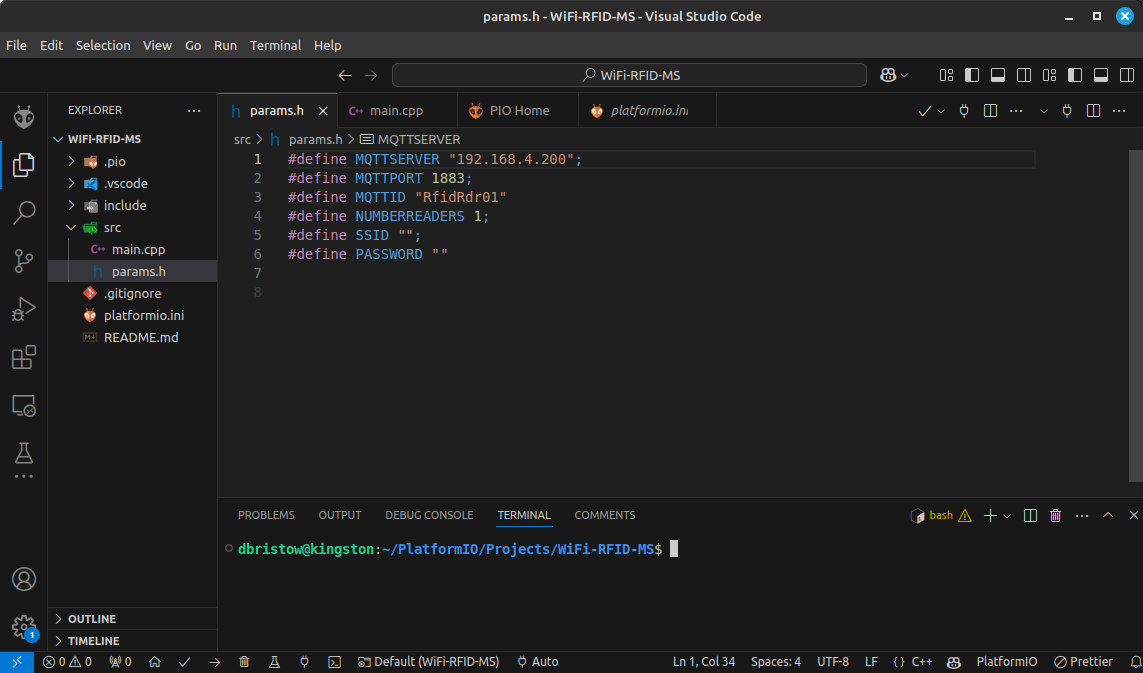
\includegraphics[scale=0.33]{./images/vsc-rfidsw.png}
    \caption{params.h File}
    \label{fig:params}
\end{figure}

\section{Building and Uploading the Code}
Once you have modified the `params.h` file with the necessary configuration parameters, you can build and upload the code to your ESP8266 board using PlatformIO. 
Follow these steps to build and upload the code:
\begin{enumerate}
    \item Connect your ESP8266 board to your computer using the micro-USB cable.
    \item Open the PlatformIO Home panel in \gls{vscode}.
    \item Select your ESP8266 board from the list of available boards. If your board is not listed, you may need to install the corresponding platform package.
    \item Click the "Build" button in the PlatformIO Home panel. This will compile the code into a binary file.
    \item Click the "Upload" button to upload the compiled code to your ESP8266 board.
\end{enumerate}
Figure \ref{fig:build} shows the `main.cpp` file with the code that will be uploaded to the ESP8266 board. Make sure to save the file before building and uploading the code.
The build icon is shown with a yellow arrow and the upload icon is shown with a green arrow in the PlatformIO Home panel.
\begin{figure}[H]
    \centering
    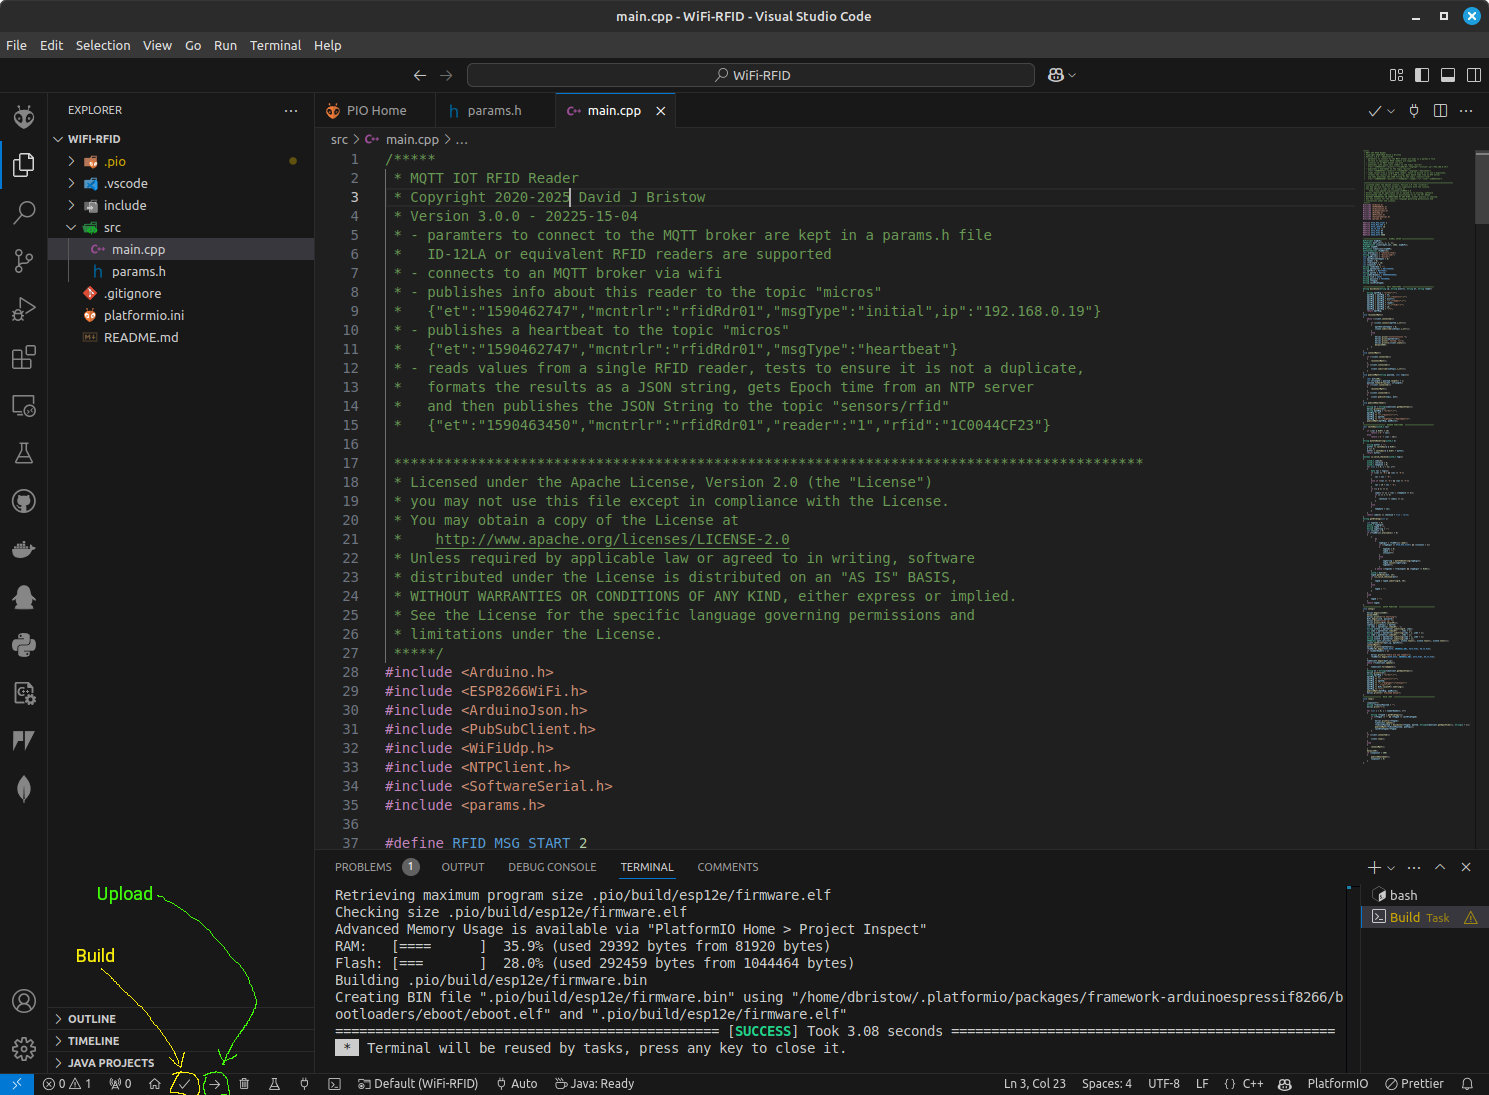
\includegraphics[scale=0.33]{./images/vsc-build.png}
    \caption{main.cpp File}
    \label{fig:build}
\end{figure}

\section{Monitoring the Serial Output (Optional)}
You can monitor the serial output of the ESP8266 board to debug any issues and observe the program's behavior. Follow these steps to monitor the serial output:
\begin{enumerate}
    \item Check that there is a \gls{rfid} reader connected to the ESP8266.
    \item Open the PlatformIO Serial Monitor in \gls{vscode}.
    \item Set the baud rate to match the baud rate used in your code (usually 115200).
    \item Observe the serial output to monitor the program's behavior and debug any issues.
    \item pass a \gls{rfid} tag over the RFID reader to see the output.
\end{enumerate}

\section{Operationalize the RFID Reader}
Once you have successfully uploaded the code to your ESP8266 board and verified that the \gls{rfid} reader is working correctly, you can start using it for your applications.
The \gls{rfid} reader will publish gls{rfid} tag data to the \gls{mqtt} broker, allowing other devices to subscribe to this data and perform various actions based on the received information.
\begin{enumerate}
    \item Install a \gls{rfid} reader under a scetion of track on your model railroad.
    \item Connect the \gls{rfid} reader to the ESP8266 board that has the code uploaded.
    \item Connect the ESP8266 board to a power source.
\end{enumerate}

